\documentclass[xcolor=pdftex,dvipsnames,table,final]{beamer}
\mode<presentation>
{
  \usetheme{PosterCERG}
}
% size in width and height is in cm
% Arch D: 24"x36" use 60.96 x 91.44 Typical size for our printer, use 3 columns, scale=0.8 to fit more text
% each column should be 0.3\linewidth
% Arch E: 36"x48" use 91.44 x 121.92 OK for FedexKinko, use 4 columns
% each column should be 0.22\linewidth
\usepackage[orientation=portrait,size=custom,width=76.2,height=106.68,scale=1]{beamerposter}
% DATE-2016 Poster format
% DIN-A0-Portrait ----1189mm X 841mm or 118.9cm x 84.1cm or 46.8in x 33.1in 
%\usepackage[orientation=portrait, size=custom, width=84.1, height=118.9 scale=1.0]{beamerposter}sd
\usepackage{multirow,wrapfig}
\usepackage[labelformat=empty,justification=centering]{caption}
\usepackage{tikz}
\usepackage{lmodern}
\usepackage{multirow}
\usepackage{listings}
\usepackage{fancyvrb}
\usepackage{lipsum}
\usetikzlibrary{fit,arrows,calc,positioning}
%\usepackage{wrapfig}
%%%%%%%%%%% Additional packages-Panci
\usepackage[utf8]{inputenc}
\usepackage[T1]{fontenc}
\usepackage{amssymb,amsmath}
\usepackage{ concrete }   

\definecolor{ocean}{RGB}{0,205,255}
\definecolor{beamerbackground}{rgb}{0.5,0.5,0.3}
\newcommand{\rb}[1]{\raisebox{1.3ex}[-1.3ex]{#1}}

\newcommand{\urlwofont}[1] { \urlstyle{same}\url{#1} }
     
\graphicspath{{figures/}}
\title{\LARGE Flexible, Opensource workBench fOr Side-channel analysis\\ \vspace{0.5ex}(FOBOS)}
\author{Abubakr Abdulgadir, William Diehl, Rajesh Velegalati, Jens-Peter Kaps}%\vspace{-2ex}
\institute{\vspace{-1ex}Department of Electrical and Computer Engineering, George Mason University, Fairfax, Virginia 22030, USA
           %\{pyalla, ehomsiri, jkaps\}@gmu.edu \url{http://cryptography.gmu.edu}
          } %this should be GMU etc. 
\date{March}

\begin{document}
\lstset{%
  basicstyle=\ttfamily,
  language=bash,
  commentstyle=\color{tabutter},
  keywordstyle=\color{black},
  numberstyle=\color{cergbg1},
  stringstyle=\color{ta3orange},
  identifierstyle=\color{cergbg1}
}
\begin{frame}[fragile]{} 
  \begin{columns}[t]
% ---------------------------------------------------------------------------
%   FIRST COLUMN
% ---------------------------------------------------------------------------
    \begin{column}{.31\linewidth}

% ---------------------------------------------------------------------------
      \begin{block}{Abstract}
Side-channel analysis attacks pose a grave threat to implementations of cryptographic 
Algorithms implemented in software as well as in hardware. 
FOBOS, an ``acquisition to analysis'' solution, includes all necessary software to control the device 
under test (attack) (DUT), trigger 
the oscilloscope, obtain the measurements and analyze them using several power analysis techniques. 
%The components of FOBOS are build in a modular fashion so that it can easily be adapted for new FPGA 
%boards, oscilloscopes, and attack techniques.
Our latest release of FOBOS has significant enhancements over
the last release announced at HOST 2016. 
The most prominent one is the capability of 
performing Test Vector Leakage Assessment (TVLA) based on Welch's t-test. This is an industry-standard
method to evaluate the effectiveness of side-channel countermeasures. 
This assessment is especially valuable in conjunction with our new profiler which ties each t-test
evaluation to the state of the cryptographic function under evaluation. This allows a user to 
pin-point during which operation information is leaking. Furthermore, FOBOS is now compatible with 
the CAESAR API, enabling evaluation of implementations on FPGAs of candidates of the 
Competition for Authenticated Encryption: Security, Applicability, and Robustness (CAESAR) without 
changes to FOBOS.
      \end{block}
	 
%---------------------------------------------------------------------------------

     

% ---------------------------------------------------------------------------
      \begin{block}{FOBOS}
        {\color{red}F}lexible {\color{red}O}pen-source work{\color{red}B}ench 
        f{\color{red}O}r {\color{red}S}ide-channel analysis, 
          loosely named after the Greek god Phobos ($\phi \acute{o} \beta o \varsigma$) is 
          an open-source framework for DPA with the following goals: 
        \begin{itemize}
          \item Complete solution useful for education.
          \item De-couples Control from Device under Test (DUT).
          \item Allows use of inexpensive FPGA boards.
          \item Modular software, allows for easy adaptation for new boards, oscilloscopes.
          \item Extensible by the user to include
          \begin{itemize}
            \item new attack scenarios and
            \item new attack models. 
          \end{itemize}
        \end{itemize}
      \end{block}
% ---------------------------------------------------------------------------
      \begin{block}{Main Components of FOBOS}
        \begin{center}
          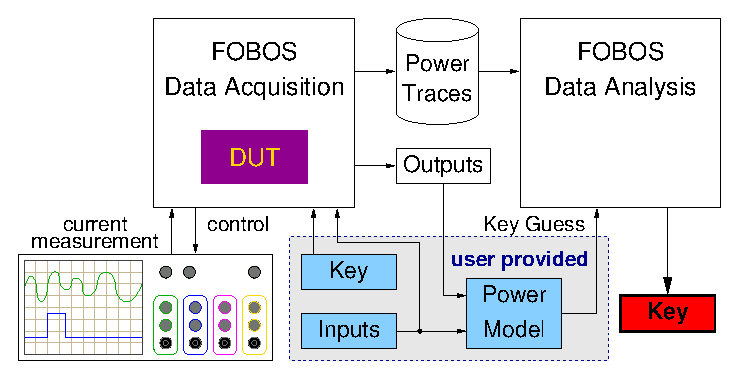
\includegraphics[scale=1.6]{../figures/fobos-top}
        \end{center} 
      \end{block}
     
 % ---------------------------------------------------------------------------
      \begin{block}{FOBOS Hardware}
        \vspace{-1ex}
        \begin{center}
          \includegraphics[width=0.9\linewidth]{../figures/FOBOSv2}
        \end{center} 
%        \begin{itemize}
%          \item FOBOS Control can be Digilent Nexys2 or Nexys3.
%        \end{itemize}
        \vspace{-0.2ex}
       \end{block}

% ---------------------------------------------------------------------------
      \begin{block}{FOBOS Acquisition}
        \begin{center}
          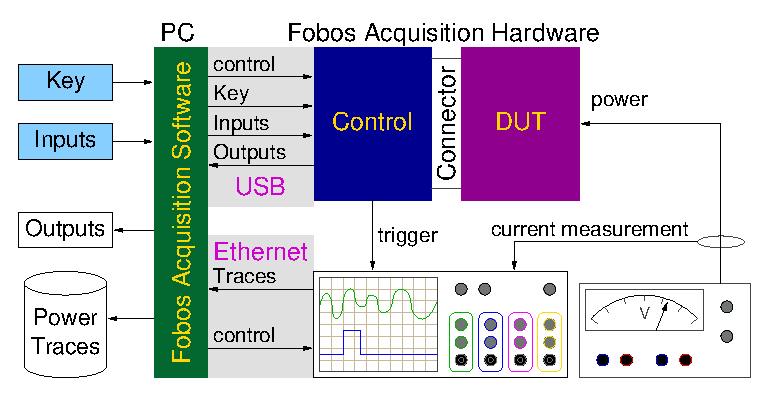
\includegraphics[scale=1.7]{../figures/fobos-dac}
        \end{center} 

          \begin{itemize}
            \item FOBOS Acquisition Hardware contains 
            \begin{itemize}
              \item VHDL for the \textbf{Control Board} to interface with DUT,
              \item VHDL-wrapper for the \textbf{DUT board} to instantiate a user provided algorithm, and
              \item Connector description.
            \end{itemize}
            \item FOBOS Acquisition Software is written in Python and 
            \begin{itemize}
              \item Controls FOBOS Acquisition Hardware,
              \item Controls measurement equipment, and
              \item Stores measurements and setup information.
            \end{itemize}
          \end{itemize}
       \end{block}
     
%---------------------------------------------------------------------------------
    \end{column}
% ---------------------------------------------------------------------------
%   SECOND COLUMN
% ---------------------------------------------------------------------------
    \begin{column}{.31\linewidth}
   
% ---------------------------------------------------------------------------
      


% ---------------------------------------------------------------------------
      \begin{block}{Acquisition Control}
        \begin{center}
          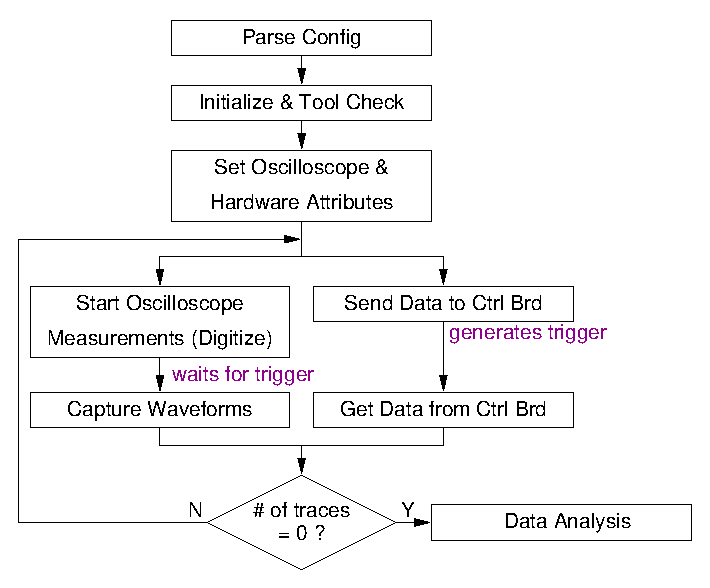
\includegraphics[scale=1.5]{../figures/data_acq}
        \end{center} 
        \begin{itemize}
          \item Control Board sends Key and Plaintext to the DUT.
          \item After DUT receives all data, the Control Board generates the trigger.
          \item The trigger indicates that the cryptographic algorithm has started
                and initiates capture of data by the oscilloscope.
        \end{itemize}
       \end{block}
     % ---------------------------------------------------------------------------
       \begin{block}{FOBOS Analysis}
        \begin{minipage}{0.69\linewidth}
		\includegraphics[scale=1.5]{../figures/fobos-dan}
        \end{minipage}
	\hspace{-5ex}
	\begin{minipage}{0.31\linewidth}
          {\small
          \begin{itemize}
            \item Minimum Guessing Entropy shows how many guesses (possible keys) are 
                  remaining for a given number of traces. 
            \item Autocorrelation indicates repeating patterns in a trace such as round 
                  operations which help in identifying where to attack. 
          \end{itemize}
          }  
	\end{minipage} 
       \end{block}
% ---------------------------------------------------------------------------
       \begin{block}{DPA Workflow}
        \vspace{-1ex}
        \begin{center}
          \includegraphics[scale=1.5]{../figures/data_anl}
        \end{center} 
        \vspace{-1ex}
        \begin{enumerate}
          \item Statistics Module
          \begin{itemize}
            \item Statistics can identify outliers in traces and samples across traces.
          \end{itemize}
          \item Post-Processing Module
          \begin{itemize}
            \item The main goal of these modules is to reduce the amount of data that 
                  has to be analyzed by the SCA Module.
          \end{itemize}
          \item SCA Module
          \begin{itemize}
            \item User can test his/her own power model using a library of state-of-the art side channel
                  distinguishers.
            \item FOBOS supports CPA using Spearman, Pearson, ANOVA \& MIA.
          \end{itemize}
        \end{enumerate}

       \end{block}
       
       \begin{block}{Example: Attack on AES}
        \vspace{-1ex}
         \begin{center}
           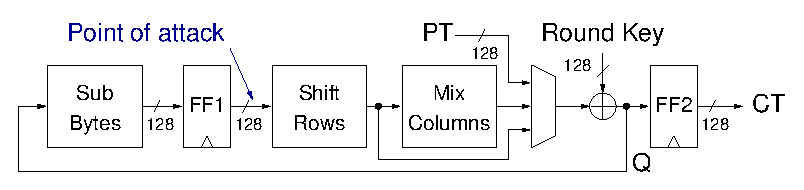
\includegraphics[width=0.9\linewidth]{../figures/aes128}

           {\small $PowerGuess_{i, j}$ = HD(SBOX($CT_{i-1}$), SBOX($PT_{i}$ $\oplus$ $KeyGuess_{j}$) )}
         \end{center}
	 \begin{minipage}[t]{0.49\linewidth}
		 %\begin{center}
			~~\includegraphics[width=0.80\linewidth]{../figures/oscilloscope-all-4ch} 
		%\end{center}
	 
	 \end{minipage}%
	 \begin{minipage}[t]{0.49\linewidth}  
		 \hspace{-5ex}\vspace{-6cm}{\small
		 \begin{itemize}
		  \item First round attack on AES-128.
		  \item Key (0x16) recovered after 1 hour.
                  \item Requires 2000 encryptions.
                  \item Pearson's Correlation.
                  \item Sometimes histogram is more clear than correlation plot.
		 \end{itemize}}
         \end{minipage} 
	 
        \begin{minipage}[t]{0.49\linewidth}
           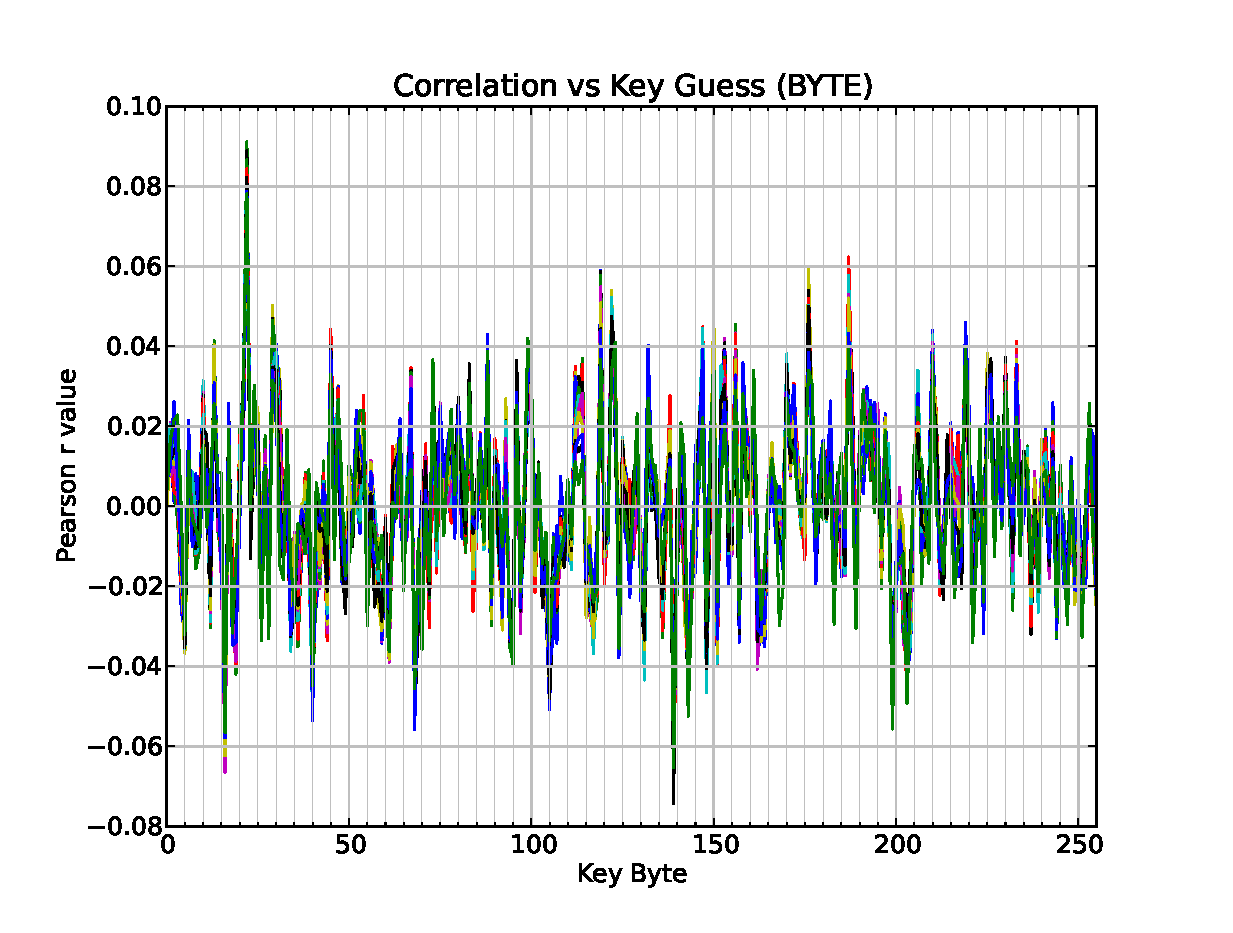
\includegraphics[width=1.0\linewidth]{../figures/pearsonsCoActual}
        \end{minipage}%
        \begin{minipage}[t]{0.49\linewidth}  
		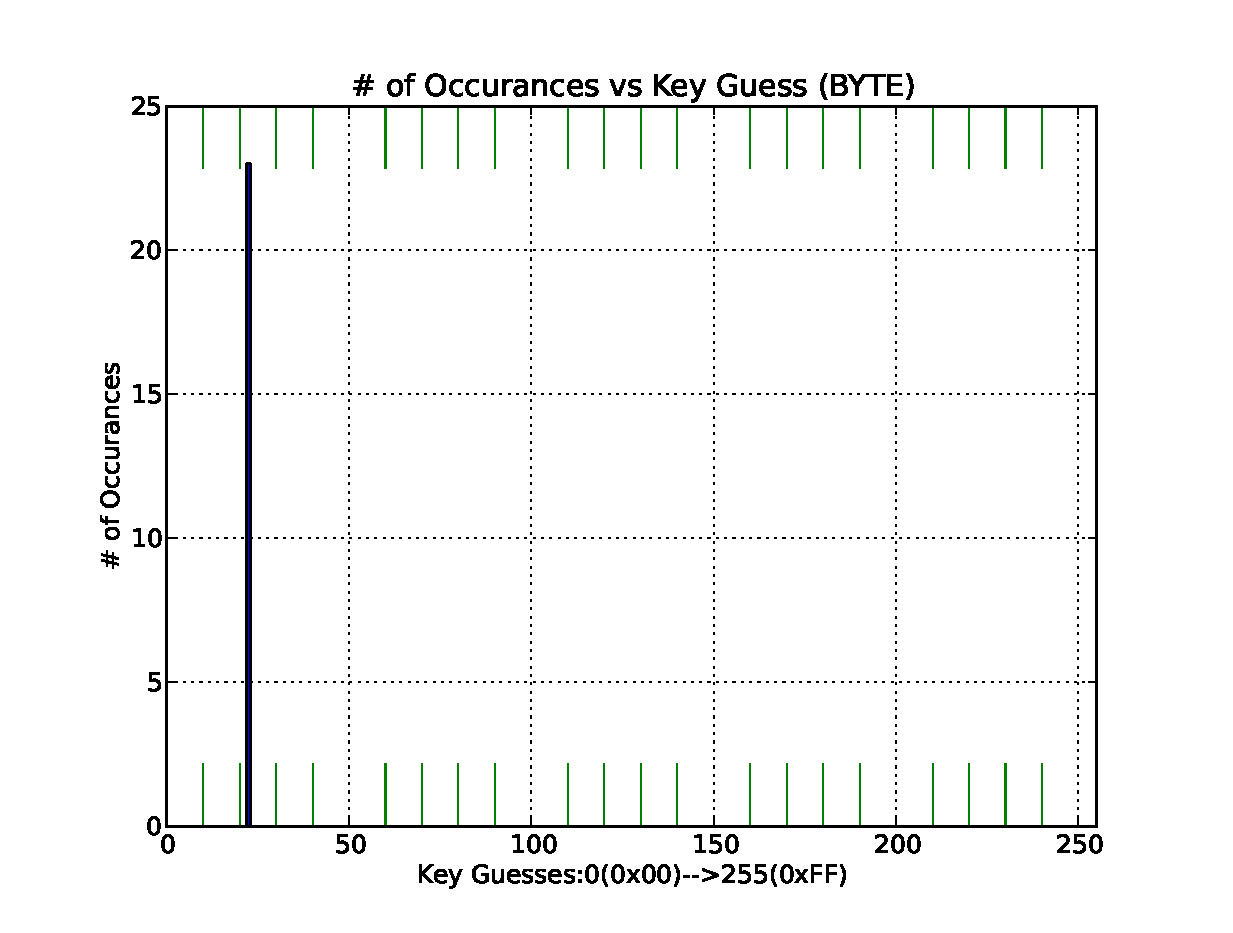
\includegraphics[width=1.0\linewidth]{../figures/histPearsonsCoActual}
        \end{minipage}
        \vspace{-3.8ex}
       \end{block}
%----------------------------------------------------------------------------
       \begin{block}{Power Measurement}
        \begin{minipage}{0.45\linewidth}
         \vspace{-0.7ex}
		\includegraphics[scale=0.9]{../figures/xbp-no-xbh}
         \vspace{-1ex}
        \end{minipage}%
%	\hspace{-5ex}
	\begin{minipage}{0.48\linewidth}
          \begin{itemize}
            \item XXBX Power Shim XBP
            \item Contains current shunt and current shunt amplifier
            \item Selectable gain: 25, 50, 100, 200
          \end{itemize}
	\end{minipage} 
       \end{block}
          
% ---------------------------------------------------------------------------
% ---------------------------------------------------------------------------
    \end{column}
% ---------------------------------------------------------------------------
%   THIRD COLUMN
% ---------------------------------------------------------------------------
   \begin{column}{.31\linewidth}
    

%----------------------------------------------------------------------------
      \begin{block}{Example: Power Measurement}
         \vspace{-1ex}
         \begin{itemize}
          \item Oscilloscope collects traces then a script calculates power consumption.
        \begin{center}
          \includegraphics[scale=0.8]{../figures/power.png}
        \end{center}
        \item Sample results:
         \end{itemize}
        \begin{center}
        \begin{minipage}[t]{0.9\linewidth}  
        \setbeamercolor{padding}{fg=white, bg=cergbg1}
        \begin{beamercolorbox}[rounded=true]{padding}
\begin{Verbatim}[fontsize=\small]
Source File: rawDataAligned.npy
Start sample (for truncated traces): 1
...
XBP Shunt Resistance (ohms): 1
...
Mean voltage for truncated traces is: 0.67885V
Mean power for truncated traces is: 0.0326W
\end{Verbatim}
        \end{beamercolorbox}
        \end{minipage}
        \end{center}


      \end{block}
%----------------------------------------------------------------------------
      \begin{block}{Welch's T-Test}
         \vspace{-1ex}
         \begin{itemize}
      \item Welch's T-test is used to evaluate DPA resistance.
      $$\frac{\mu_0 - \mu_1}{\sqrt{\frac{s_0^2}{n_0}+ \frac{s_0^2}{n_0}}} 
         \quad p = 2 \int_{|t|}^\infty f(t,v) \mathrm{d}t $$
      $$ p = 2F(-4.5,v > 10000) < -0.00001$$
         \end{itemize}
         \begin{minipage}{0.4\linewidth}
        \begin{center}
     \includegraphics[scale=1.5]{../figures/t-test-flow}
        \end{center} 
        \end{minipage}
         \begin{minipage}{0.5\linewidth}
      {\small
          Where $\mu_0$ and $\mu_1$ are means of distributions 0 and 1, s0 and s1 are standard deviations, and n0 and n1 are the cardinality of the distributions, or the number of samples.
          }
         \begin{itemize}
           \item Finds leakage without attack.
           \item T-test fails if $|t| > 4.5$\\ $\Rightarrow$ {\color{red}design leaks}.
           \item No power model needed.
           \item No knowledge of architecture needed.
         \end{itemize}
        \end{minipage}
         
      \end{block}
%----------------------------------------------------------------------------
      \begin{block}{Example: T-Test on AES-GCM Implementation}
         \begin{minipage}{0.45\linewidth}
             \begin{center}
               Fail: Unprotected
            \includegraphics[scale=0.6]{../figures/aes_gcm_unprotected.png}
        \end{center} 
        \end{minipage}
       \begin{minipage}{0.45\linewidth}

        \begin{center}
             Pass: Protected
            \includegraphics[scale=0.6]{../figures/aes_gcm_protected.png}
            \end{center} 
         
        \end{minipage}
        
         
      \end{block}

%----------------------------------------------------------------------------
      \begin{block}{Profiler}
         \begin{itemize}
           \item \textbf{Problem:} It is difficult to correlate leakage points to operations on the DUT.
           \item \textbf{Solution:} \emph{Profiler} maps DUT state to samples in power trace.
           \item \textbf{Example}: Determining leakage points in AES-CLOC implementation's t-test result:
         \begin{itemize}
         \item T-test detects leakage at discrete points:
          \begin{center}
          \includegraphics[scale=0.254]{../figures/profiler_1.png}
          \end{center}
          \item After zooming into a spike, we can see the DUT state at that time:
     \begin{center}
          \includegraphics[scale=0.254]{../figures/profiler_2.png}
          \end{center}
          \item Reason for the spike: CLOC has a data-dependent branch condition (from the CLOC specification).
          \newline
          \begin{center}
          \includegraphics[scale=1.2]{../figures/cloc_aes_branch.png}
           \end{center}

         \end{itemize}

         \end{itemize}
       
       
          
    
         
      \end{block}
% ---------------------------------------------------------------------------
% ---------------------------------------------------------------------------
%      \begin{block}{References}
%        \footnotesize
%          \bibliographystyle{IEEEtran}
%          \bibliography{keccak}
%        %\input{keccakbib}
%      \end{block} 
   \end{column}
\end{columns}

\end{frame}
\end{document}

 
